%%%%%%%%%%%%%%%%%%%%%%%%%%%%%%%%%%%%%%%%%%%%%%%%%%%%%%%%%%%%%%%%%%%%%%%%%%%%%%%%%%
\begin{frame}[fragile]\frametitle{}
\begin{center}
{\Large Linear Regression with Scikit-Learn}
\end{center}
\end{frame}


%%%%%%%%%%%%%%%%%%%%%%%%%%%%%%%%%%%%%%%%%%%%%%%%%%%%%%%%%%%%%%%%%%%%%%%%
\begin{frame}[fragile]\frametitle{Linear Regression}
\begin{lstlisting}
import pandas
from sklearn import model_selection
from sklearn.linear_model import LinearRegression
url = "https://raw.githubusercontent.com/jbrownlee/Datasets/master/housing.data"
names = ['CRIM', 'ZN', 'INDUS', 'CHAS', 'NOX', 'RM', 'AGE', 'DIS', 'RAD', 'TAX', 'PTRATIO', 'B', 'LSTAT', 'MEDV']
dataframe = pandas.read_csv(url, delim_whitespace=True, names=names)
array = dataframe.values
X = array[:,0:13]
Y = array[:,13]
seed = 7
kfold = model_selection.KFold(n_splits=10, random_state=seed)
model = LinearRegression()
scoring = 'neg_mean_absolute_error'
results = model_selection.cross_val_score(model, X, Y, cv=kfold, scoring=scoring)
print("MAE: %.3f (%.3f)") % (results.mean(), results.std())

MAE: -4.005 (2.084)
\end{lstlisting}

{\tiny (Ref: Metrics To Evaluate Machine Learning Algorithms in Python - Jason Brownlee)}

\end{frame}


% %%%%%%%%%%%%%%%%%%%%%%%%%%%%%%%%%%%%%%%%%%%%%%%%%%%%%%%%%%%%%%%%%%%%%%%%
% \begin{frame}[fragile]\frametitle{Template code for Linear Regression}
% \begin{lstlisting}
% from sklearn import linear_model 

% x_train=input_variables_values_training_datasets 
% y_train=target_variables_values_training_datasets 
% x_test=input_variables_values_test_datasets 

% linear = linear_model.LinearRegression() 

% linear.fit(x_train, y_train) 
% linear.score(x_train, y_train) 

% print('Coefficient: \n', linear.coef_) 
% print('Intercept: \n', linear.intercept_) 

% predicted= linear.predict(x_test)
% \end{lstlisting}
% \end{frame}



% %%%%%%%%%%%%%%%%%%%%%%%%%%%%%%%%%%%%%%%%%%%%%%%%%%%%%%%%%%%%%%%%%%%%%%%%
% \begin{frame}[fragile]\frametitle{Artificial Data Creation}
% % Fitting a line to sample $ (x,y)$ data
% \begin{lstlisting}
% import matplotlib.pyplot as plt
% import numpy as np

% rng = np.random.RandomState(42)
% x = 10 * rng.rand(50)
% y = 2 * x - 1 + rng.randn(50)
% plt.scatter(x, y);
% \end{lstlisting}
% \begin{center}
% 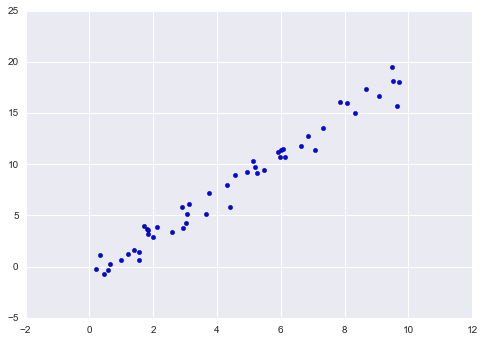
\includegraphics[width=0.5\linewidth]{regrex1}
% \end{center}
% \end{frame}



% %%%%%%%%%%%%%%%%%%%%%%%%%%%%%%%%%%%%%%%%%%%%%%%%%%%%%%%%%%%%%%%%%%%%%%%%
% \begin{frame}[fragile]\frametitle{Data Arrangement}
% \begin{itemize}
% \item Arrange data into a features matrix and target vector.
% \item Requires a two-dimensional features matrix and a one-dimensional target array.
% \item Simple reshaping: \lstinline|X = x[:, np.newaxis]|
% \end{itemize}
% \end{frame}

% %%%%%%%%%%%%%%%%%%%%%%%%%%%%%%%%%%%%%%%%%%%%%%%%%%%%%%%%%%%%%%%%%%%%%%%%
% \begin{frame}[fragile]\frametitle{Model Selection}
% \begin{itemize}
% \item For a simple linear regression model use: \lstinline|from sklearn.linear_model import LinearRegression|
% \item Choose model hyperparameters \lstinline|model = LinearRegression(fit_intercept=True)|
% \item Documentation:
% \begin{lstlisting}
% LinearRegression(copy_X=True, fit_intercept=True, n_jobs=1, normalize=False)
% \end{lstlisting}
% \end{itemize}
% \end{frame}

% %%%%%%%%%%%%%%%%%%%%%%%%%%%%%%%%%%%%%%%%%%%%%%%%%%%%%%%%%%%%%%%%%%%%%%%%
% \begin{frame}[fragile]\frametitle{Training}
% \begin{itemize}
% \item Fit the model to your data \lstinline|model.fit(X, y)|
% \item This fit() causes many internal computations to take place, and the results are stored in \lstinline|model.coef_| and \lstinline|model.intercept_|
% \item These two parameters represent the slope and intercept of the simple linear fit to the data. 
% \end{itemize}
% \end{frame}

% %%%%%%%%%%%%%%%%%%%%%%%%%%%%%%%%%%%%%%%%%%%%%%%%%%%%%%%%%%%%%%%%%%%%%%%%
% \begin{frame}[fragile]\frametitle{Model Parameters}
% \begin{itemize}
% \item During the fitting process, the state of the estimator is stored in instance attributes that have a trailing underscore ('\_'). 
% \item For example, the coefficients of a LinearRegression estimator are stored in the attribute \texttt{coef\_}:
% \end{itemize}

% \begin{lstlisting}
% est.coef_   # access coefficients
% # Output : array([ 0.33176871,  0.34910639])
% \end{lstlisting}
% \end{frame}


% %%%%%%%%%%%%%%%%%%%%%%%%%%%%%%%%%%%%%%%%%%%%%%%%%%%%%%%%%%%%%%%%%%%%%%%%
% \begin{frame}[fragile]\frametitle{Testing}
% \begin{itemize}
% \item Predict labels for unknown data \lstinline|xtest = np.linspace(-1, 11)|
% \item Similar to training data this unseen data also needs to be reshaped into required matrix form
% \begin{lstlisting}
% Xtst = xtest[:, np.newaxis]
% ytst = model.predict(Xtst)
% \end{lstlisting}
% \item Visualize \lstinline|plt.plot(Xtst, ytst);|
% \end{itemize}
% \end{frame}

% %%%%%%%%%%%%%%%%%%%%%%%%%%%%%%%%%%%%%%%%%%%%%%%%%%%%%%%%%%%%%%%%%%%%%%%%
% \begin{frame}[fragile]\frametitle{Simple linear regression}
% \begin{center}
% 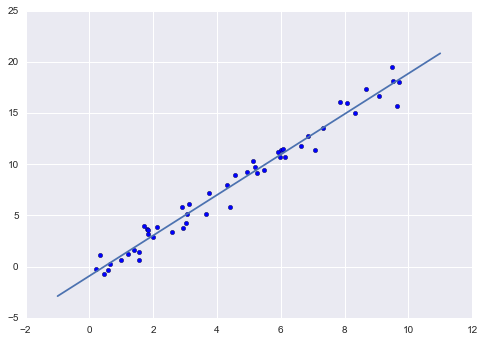
\includegraphics[width=0.9\linewidth]{regrex2}
% \end{center}
% \end{frame}

% %%%%%%%%%%%%%%%%%%%%%%%%%%%%%%%%%%%%%%%%%%%%%%%%%%%%%%%%%%%%%%%%%%%%%%%%
% \begin{frame}[fragile]\frametitle{Extended Exercise}
% \begin{itemize}
% \item Make current x list of values as x1
% \item Create another list as x2 (same dimensions!!)
% \item Incorporate both x1 and x2 in X
% \item Build the model
% \item Make appropriate changes while testing.
% \end{itemize}
% \end{frame}


% %%%%%%%%%%%%%%%%%%%%%%%%%%%%%%%%%%%%%%%%%%%%%%%%%%%%%%%%%%%%%%%%%%%%%%%%%
% %\begin{frame}[fragile]\frametitle{Another Example}
% %
% %\begin{lstlisting}
% %from sklearn.linear_model import LinearRegression
% %import numpy as np
% %
% %# random training data
% %X = np.random.rand(10, 2)
% %y = np.random.randint(2, size=10)
% %
% %est = LinearRegression(fit_intercept=False)
% %est.fit(X, y)
% %\end{lstlisting}
% %\end{frame}
% %


% %%%%%%%%%%%%%%%%%%%%%%%%%%%%%%%%%%%%%%%%%%%%%%%%%%%%%%%%%%%%%%%%%%%%%%%%%%%%%%%%%%
% \begin{frame}[fragile]\frametitle{}
% \begin{center}
% {\Large Test Case: Glass Identification }
% \end{center}
% \end{frame}

% %%%%%%%%%%%%%%%%%%%%%%%%%%%%%%%%%%%%%%%%%%%%%%%%%%%%%%%%%%%%%%%%%%%%%%%%
% \begin{frame}[fragile]\frametitle{Glass identification Dataset}
% \begin{itemize}
% \item Toy Dataset:  http://archive.ics.uci.edu/ml/machine-learning-databases/glass/glass.data
% \item  Pretend that we want to predict ri, and our only feature is al. How could we do it using machine learning?
% \end{itemize}
% %\begin{lstlisting}
% %import pandas as pd
% %advertising = pd.read_csv('../data/Advertising.csv')
% %advertising.head(5)
% %\end{lstlisting}
% \begin{center}
% 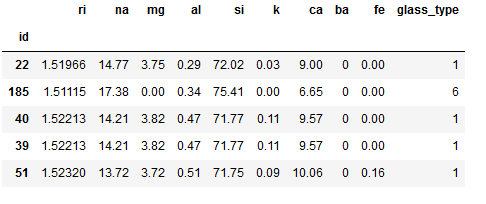
\includegraphics[width=0.9\linewidth]{glassdt}
% \end{center}
% \end{frame}



% %%%%%%%%%%%%%%%%%%%%%%%%%%%%%%%%%%%%%%%%%%%%%%%%%%%%%%%%%%%%%%%%%%%%%%%%
% \begin{frame}[fragile]\frametitle{Example: Glass identification Dataset}
% \begin{lstlisting}
% import pandas as pd
% col_names = ['id','ri','na','mg','al','si','k','ca','ba','fe','glass_type']
% glass = pd.read_csv('glass.data', names=col_names, index_col='id')
% glass.sort('al', inplace=True)
% print(glass.head())
% \end{lstlisting}
% \end{frame}

% %%%%%%%%%%%%%%%%%%%%%%%%%%%%%%%%%%%%%%%%%%%%%%%%%%%%%%%%%%%%%%%%%%%%%%%
% \begin{frame}[fragile]\frametitle{Example: Glass identification Dataset}
% \begin{center}
% 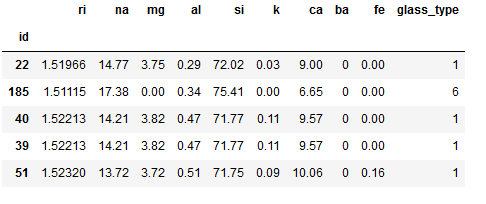
\includegraphics[width=0.9\linewidth]{glassdt}
% \end{center}
% %\tiny
% \begin{itemize}
% \item Question: Pretend that we want to predict ri, and our only feature is al. How could we do it using machine learning?
% \item Answer: We could frame it as a regression problem, and use a linear regression model with al as the only feature and ri as the response.
% \end{itemize}
% \end{frame}

% %%%%%%%%%%%%%%%%%%%%%%%%%%%%%%%%%%%%%%%%%%%%%%%%%%%%%%%%%%%%%%%%%%%%%%%
% \begin{frame}[fragile]\frametitle{Glass identification Dataset}
% \begin{itemize}
% \item Question: How would we visualize this model?
% \item Answer: Create a scatter plot with al on the x-axis and ri on the y-axis, and draw the line of best fit.
% \end{itemize}
% \end{frame}

% %%%%%%%%%%%%%%%%%%%%%%%%%%%%%%%%%%%%%%%%%%%%%%%%%%%%%%%%%%%%%%%%%%%%%%%
% \begin{frame}[fragile]\frametitle{Glass identification Dataset}
% \begin{lstlisting}
% import seaborn as sns
% import matplotlib.pyplot as plt

% sns.set(font_scale=1.5)
% sns.lmplot(x='al', y='ri', data=glass, ci=None)
% \end{lstlisting}
% \begin{center}
% 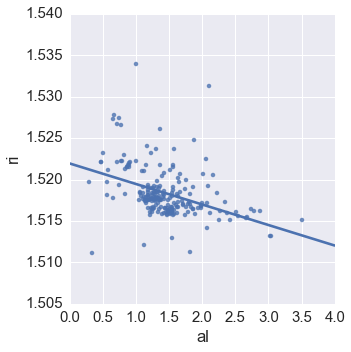
\includegraphics[width=0.45\linewidth]{glasssns}
% \end{center}
% \end{frame}


% %%%%%%%%%%%%%%%%%%%%%%%%%%%%%%%%%%%%%%%%%%%%%%%%%%%%%%%%%%%%%%%%%%%%%%%
% \begin{frame}[fragile]\frametitle{Glass identification Dataset}
% Without using Seaborn? Use Plot from Pandas
% \begin{lstlisting}
% # scatter plot using Pandas
% glass.plot(kind='scatter', x='al', y='ri')
% \end{lstlisting}
% \begin{center}
% 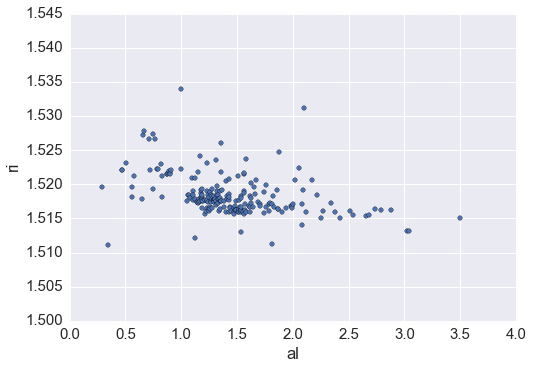
\includegraphics[width=0.6\linewidth]{glasspd}
% \end{center}
% \end{frame}

% %%%%%%%%%%%%%%%%%%%%%%%%%%%%%%%%%%%%%%%%%%%%%%%%%%%%%%%%%%%%%%%%%%%%%%%
% \begin{frame}[fragile]\frametitle{Glass identification Dataset}
% In Matplotlib?
% \begin{lstlisting}
% # equivalent scatter plot using Matplotlib
% plt.scatter(glass.al, glass.ri)
% plt.xlabel('al')
% plt.ylabel('ri')
% \end{lstlisting}
% \begin{center}
% 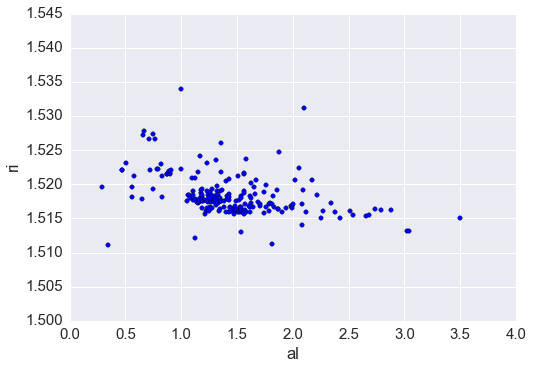
\includegraphics[width=0.6\linewidth]{glassplt}
% \end{center}
% \end{frame}



% %%%%%%%%%%%%%%%%%%%%%%%%%%%%%%%%%%%%%%%%%%%%%%%%%%%%%%%%%%%%%%%%%%%%%%%
% \begin{frame}[fragile]\frametitle{Linear Regression Model}
% \begin{lstlisting}
% from sklearn.linear_model import LinearRegression

% linreg = LinearRegression()
% feature_cols = ['al']
% X = glass[feature_cols]
% y = glass.ri

% linreg.fit(X, y)

% glass['ri_pred'] = linreg.predict(X)

% print(glass.head())
% \end{lstlisting}
% \end{frame}

% %%%%%%%%%%%%%%%%%%%%%%%%%%%%%%%%%%%%%%%%%%%%%%%%%%%%%%%%%%%%%%%%%%%%%%%
% \begin{frame}[fragile]\frametitle{Linear Regression Model}
% \begin{center}
% 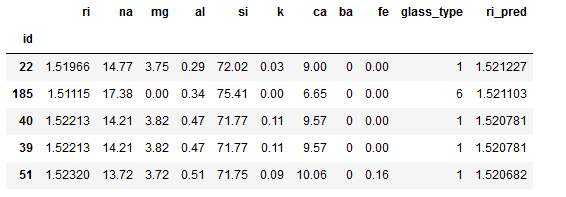
\includegraphics[width=0.9\linewidth]{glasspred}
% \end{center}
% \end{frame}

% %%%%%%%%%%%%%%%%%%%%%%%%%%%%%%%%%%%%%%%%%%%%%%%%%%%%%%%%%%%%%%%%%%%%%%%
% \begin{frame}[fragile]\frametitle{Plot}
% \begin{lstlisting}
% # plot those predictions connected by a line
% plt.plot(glass.al, glass.ri_pred, color='red')
% plt.xlabel('al')
% plt.ylabel('Predicted ri')
% \end{lstlisting}
% \begin{center}
% 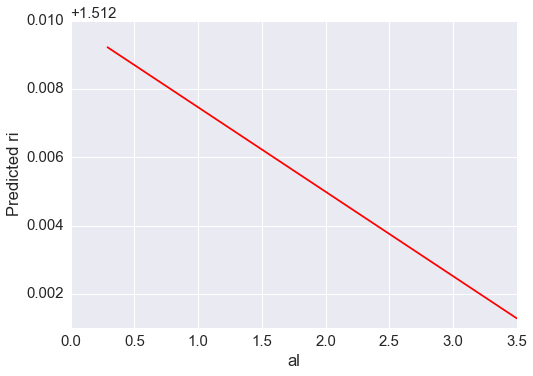
\includegraphics[width=0.6\linewidth]{glasspredplot}
% \end{center}
% \end{frame}

% %%%%%%%%%%%%%%%%%%%%%%%%%%%%%%%%%%%%%%%%%%%%%%%%%%%%%%%%%%%%%%%%%%%%%%%
% \begin{frame}[fragile]\frametitle{Plot}
% \begin{lstlisting}
% # put the plots together
% plt.scatter(glass.al, glass.ri)
% plt.plot(glass.al, glass.ri_pred, color='red')
% plt.xlabel('al')
% plt.ylabel('ri')
% \end{lstlisting}
% \begin{center}
% 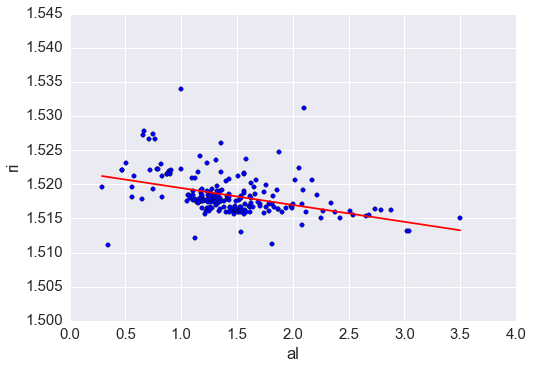
\includegraphics[width=0.6\linewidth]{glasspredplottog}
% \end{center}
% \end{frame}

% %%%%%%%%%%%%%%%%%%%%%%%%%%%%%%%%%%%%%%%%%%%%%%%%%%%%%%%%%%%%%%%%%%%%%%%
% \begin{frame}[fragile]\frametitle{Refresher: interpreting linear regression coefficients}

% Linear regression equation: $ y = \beta_0 + \beta_1 x$
% \begin{lstlisting}
% # compute prediction for al=2 using the equation
% linreg.intercept_ + linreg.coef_ * 2 
% # array([ 1.51699012])

% # compute prediction for al=2 using the predict method
% linreg.predict(2) 
% # array([ 1.51699012])

% # examine coefficient for al
% zip(feature_cols, linreg.coef_) 
% # [('al', -0.002477606387469623)]
% \end{lstlisting}
% Interpretation: 1 unit increase in 'al' is associated with a 0.0025 unit decrease in 'ri'.
% \end{frame}

% % %%%%%%%%%%%%%%%%%%%%%%%%%%%%%%%%%%%%%%%%%%%%%%%%%%%%%%%%%%%%%%%%%%%%%%%%%%%%%%%%%%
% % \begin{frame}[fragile]\frametitle{}
% % \begin{center}
% % {\Large Test Case: Advertising Budgets }
% % \end{center}
% % \end{frame}

% % %%%%%%%%%%%%%%%%%%%%%%%%%%%%%%%%%%%%%%%%%%%%%%%%%%%%%%%%%%%%%%%%%%%%%%%%
% % \begin{frame}[fragile]\frametitle{Advertising Dataset}
% % \begin{itemize}
% % \item Toy Dataset: Advertising, Advertising.csv
% % \item Sales totals for a product in 200 different markets. Advertising budget in each market, broken down into TV, radio, newspaper
% % \end{itemize}
% % %\begin{lstlisting}
% % %import pandas as pd
% % %advertising = pd.read_csv('../data/Advertising.csv')
% % %advertising.head(5)
% % %\end{lstlisting}
% % \begin{center}
% % 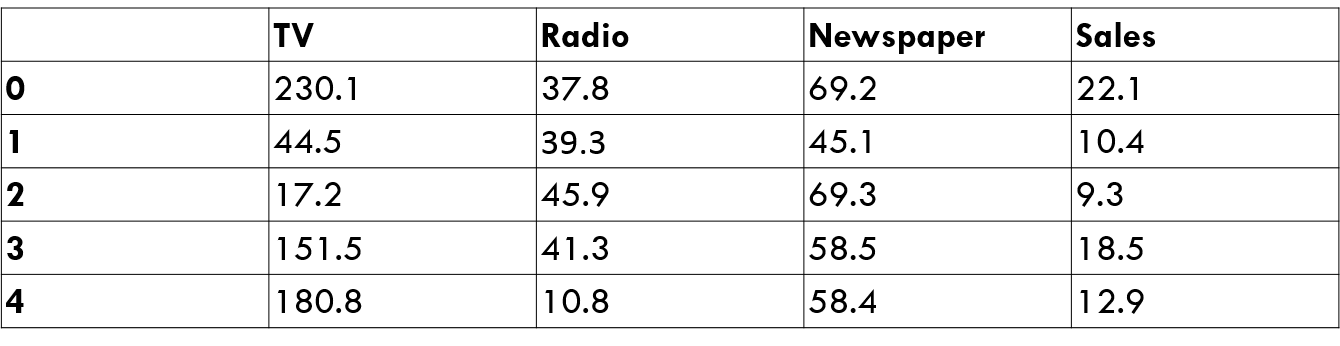
\includegraphics[width=0.8\linewidth]{advtdata}
% % \end{center}
% % \end{frame}


% % %%%%%%%%%%%%%%%%%%%%%%%%%%%%%%%%%%%%%%%%%%%%%%%%%%%%%%%%%%%%%%%%%%%%%%%%
% % \begin{frame}[fragile]\frametitle{Problem}
% % \begin{itemize}
% % \item Goal: What marketing plan for next year will result in high product sales?
% % \item Questions (Hypothesis):
	% % \begin{itemize}
	% % \item Is there a relationship between advertising budget and sales?
	% % \item How strong is the relationship between advertising budget and sales?
	% % \item Which media contribute to sales?
	% % \item How accurately can we estimate the effect of each medium on sales?
	% % \item Is the relationship linear?
	% % \item Is there any interaction effect? (called ``synergy'' in business). Example: spending 50k on TV ads + 50k on radio ads results in more sales than spending 100k on only TV
	% % \end{itemize}
% % \end{itemize}
% % \end{frame}

% % %%%%%%%%%%%%%%%%%%%%%%%%%%%%%%%%%%%%%%%%%%%%%%%%%%%%%%%%%%%%%%%%%%%%%%%%
% % \begin{frame}[fragile]\frametitle{Advertising Dataset}
% % \begin{itemize}
% % \item What are some ways we can regress sales onto adverting using Simple Linear Regression?
% % \item One model:
% % \begin{align*}
% % sales & \approx \beta_0 +  \beta_1 \times TV \\
% % y & \approx \beta_0 + \beta_1 x
% % \end{align*}
% % \item Scatter plot visualization for TV and Sales.
% % \begin{lstlisting}
% % %matplotlib inline
% % advertising.plot.scatter(x='TV', y='Sales');
% % \end{lstlisting}
% % \begin{center}
% % 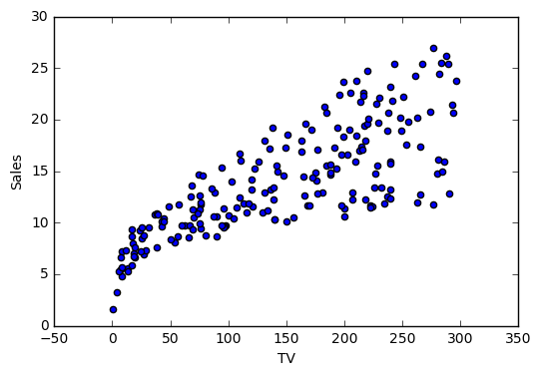
\includegraphics[width=0.4\linewidth]{advtscatter}
% % \end{center}
% % \end{itemize}
% % \end{frame}

% % %%%%%%%%%%%%%%%%%%%%%%%%%%%%%%%%%%%%%%%%%%%%%%%%%%%%%%%%%%%%%%%%%%%%%%%%
% % \begin{frame}[fragile]\frametitle{Advertising Dataset}
% % \begin{itemize}
% % \item Simple Linear Model in Python (using pandas and scikit): Predictor: $x$, Response: $y$
% % \begin{lstlisting}
% % reg = linear_model.LinearRegression()
% % reg.fit(advertising['TV'].reshape(-1,1), advertising['Sales'].reshape(-1,1))
% % print('Coefficients: \n', reg.coef_)
% % print('Intercept: \n', reg.intercept_)

% % Coefficients: [[ 0.04753664]] 
% % Intercept: [ 7.03259355]
% % \end{lstlisting}
% % \item $Sales = 7.03259 + 0.04754  \times  TV$
% % \end{itemize}
% % \end{frame}

% % %%%%%%%%%%%%%%%%%%%%%%%%%%%%%%%%%%%%%%%%%%%%%%%%%%%%%%%%%%%%%%%%%%%%%%%%
% % \begin{frame}[fragile]\frametitle{Advertising Dataset}
% % Scatter plot visualization for TV and Sales with Linear Model.
% % \begin{lstlisting}
% % plt.scatter(advertising['TV'], advertising['Sales'],  color='black')
% % plt.plot(advertising['TV'], reg.predict(advertising['TV'].reshape(-1,1)), 
        % % color='blue', linewidth=3)

% % \end{lstlisting}
% % \begin{center}
% % 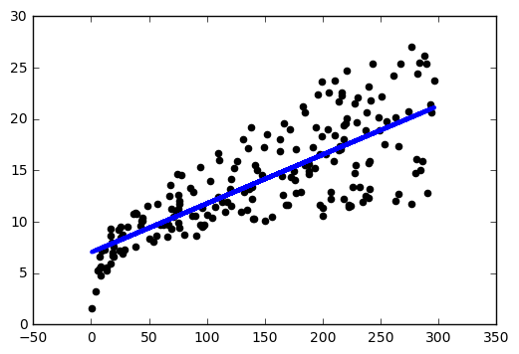
\includegraphics[width=0.6\linewidth]{advtscatterline}
% % \end{center}
% % \end{frame}


% % %%%%%%%%%%%%%%%%%%%%%%%%%%%%%%%%%%%%%%%%%%%%%%%%%%%%%%%%%%%%%%%%%%%%%%%%%%%%%%%%%%
% % \begin{frame}[fragile]\frametitle{}
% % \begin{center}
% % {\Large Test Case: Loan Disbursement}
% % \end{center}
% % \end{frame}


% %%%%%%%%%%%%%%%%%%%%%%%%%%%%%%%%%%%%%%%%%%%%%%%%%%%%%%%%%%%%%%%%%%%%%%%%%
% %\begin{frame}[fragile]\frametitle{Assignment: Line fitting on real data}
% %
% %\begin{itemize}
% %\item The Lending Club is a peer-to-peer lending site where members make loans to each other. 
% %\item The site makes anonymized data on loans and borrowers publicly available.
% %\item Just look at how borrower FICO score affects interest rate charged.
% %\item {\bf Implement:} Load the csv in pandas and plot FICO score and Interest Rate.
% %\end{itemize}
% %
% %\end{frame}
% %
% %%%%%%%%%%%%%%%%%%%%%%%%%%%%%%%%%%%%%%%%%%%%%%%%%%%%%%%%%%%%%%%%%%%%%%%%%
% %\begin{frame}[fragile]\frametitle{Line fitting on real data}
% %
% %\begin{lstlisting}
% %import pandas as pd
% %df = pd.read_csv('../data/loanf.csv')
% %
% %intrate = df['Interest.Rate']
% %fico = df['FICO.Score']
% %p = plot(fico,intrate,'o')
% %ax = gca()
% %xt = ax.set_xlabel('FICO Score')
% %yt = ax.set_ylabel('Interest Rate %')
% %\end{lstlisting}
% %\end{frame}
% %
% %%%%%%%%%%%%%%%%%%%%%%%%%%%%%%%%%%%%%%%%%%%%%%%%%%%%%%%%%%%%%%%%%%%%%%%%%
% %\begin{frame}[fragile]\frametitle{Line fitting on real data}
% %\begin{center}
% %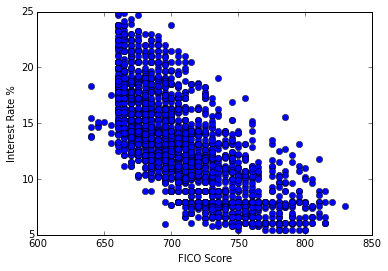
\includegraphics[width=0.9\linewidth]{loan1}
% %\end{center}
% %\end{frame}
% %
% %
% %%%%%%%%%%%%%%%%%%%%%%%%%%%%%%%%%%%%%%%%%%%%%%%%%%%%%%%%%%%%%%%%%%%%%%%%%
% %\begin{frame}[fragile]\frametitle{Line fitting on real data}
% %\begin{center}
% %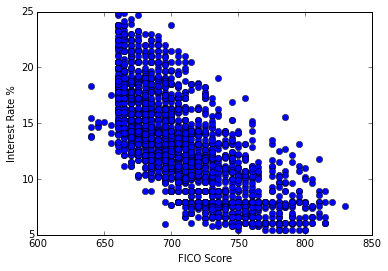
\includegraphics[width=0.5\linewidth]{loan1}
% %\end{center}
% %\begin{itemize}
% %\item Here we see a distinct downward linear trend where Interest Rate goes down with increasing FICO score. 
% %\item But we also see that for the same FICO score there is a range of Interest rates.
% %\item This suggests that FICO by itself might not be enough to predict Interest Rate.
% %\end{itemize}
% %\end{frame}
% %
% %%%%%%%%%%%%%%%%%%%%%%%%%%%%%%%%%%%%%%%%%%%%%%%%%%%%%%%%%%%%%%%%%%%%%%%%%
% %\begin{frame}[fragile]\frametitle{How can I predict?}
% %How can I predict interest rates based on borrower and loan attributes? 
% %
% %Steps:
% %\begin{itemize}
% %\item Browse the data
% %\item Data cleanup
% %\item Visual exploration
% %\item Model derivation
% %\end{itemize}
% %%\begin{center}
% %%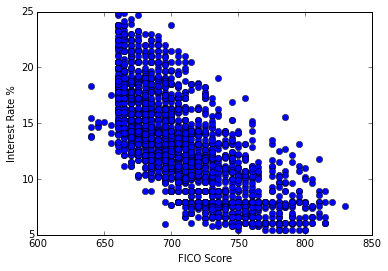
\includegraphics[width=0.5\linewidth]{loan1}
% %%\end{center}
% %\end{frame}
% %
% %%%%%%%%%%%%%%%%%%%%%%%%%%%%%%%%%%%%%%%%%%%%%%%%%%%%%%%%%%%%%%%%%%%%%%%%%
% %\begin{frame}[fragile]\frametitle{Browse Data}
% %{\bf ToDo:} Find all the variables, their data types, their ranges, meanings, etc.
% %\end{frame}
% %
% %
% %%%%%%%%%%%%%%%%%%%%%%%%%%%%%%%%%%%%%%%%%%%%%%%%%%%%%%%%%%%%%%%%%%%%%%%%%
% %\begin{frame}[fragile]\frametitle{Browse Data}
% %\begin{itemize}
% %\item Amount.Requested - numeric. The amount (in dollars) requested in the loan application.
% %\item Amount.Funded.By.Investors - numeric. The amount (in dollars) loaned to the individual.
% %\item Interest.rate - character. The lending interest rate charged to the borrower.
% %\item Loan.length - character. The length of time (in months) of the loan.
% %\item Loan.Purpose - categorical variable. The purpose of the loan as stated by the applicant.
% %\item FICO.range - categorical (expressed as a string label e.g. ``650-655''). A range indicating the applicants FICO score.
% %\end{itemize}
% %\end{frame}
% %
% %%%%%%%%%%%%%%%%%%%%%%%%%%%%%%%%%%%%%%%%%%%%%%%%%%%%%%%%%%%%%%%%%%%%%%%%
% %\begin{frame}[fragile]\frametitle{Data Cleanup}
% %We find the data are ''messy'' i.e aren't cleanly prepared for import - for instance numeric columns might have some strings in them. 
% %\begin{lstlisting}
% %import pandas as pd
% %loansData = pd.read_csv('https://spark-public.s3.amazonaws.com/dataanalysis/loansData.csv')
% %print(loansData['Interest.Rate'][0:5]) # first five rows of Interest.Rate
% %
% %81174     8.90%
% %99592    12.12%
% %80059    21.98%
% %15825     9.99%
% %33182    11.71%
% %\end{lstlisting}
% %\end{frame}
% %


% %%%%%%%%%%%%%%%%%%%%%%%%%%%%%%%%%%%%%%%%%%%%%%%%%%%%%%%%%%%%%%%%%%%%%%%%%
% %\begin{frame}[fragile]\frametitle{Credit Card Fraud}
% %\begin{itemize}
% %\item We can also think of classification as a function estimation problem where the function that we want to estimate separates the two classes. 
% %\item This is illustrated in the example below where our goal is to predict whether or not a credit card transaction is fraudulent
% %\item he dataset is provided by James et al., \textbf{Introduction to Statistical Learning}.
% %\end{itemize}
% %\end{frame}
% %
% %%%%%%%%%%%%%%%%%%%%%%%%%%%%%%%%%%%%%%%%%%%%%%%%%%%%%%%%%%%%%%%%%%%%%%%%%
% %\begin{frame}[fragile]\frametitle{Credit Card Fraud}
% %\begin{center}
% %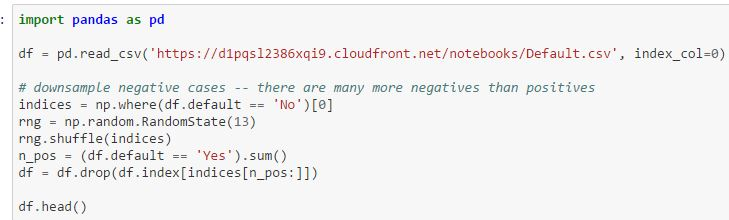
\includegraphics[width=\linewidth]{sklclass1}
% %\end{center}
% %\begin{center}
% %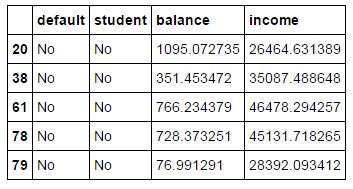
\includegraphics[width=0.5\linewidth]{sklclass2}
% %\end{center}
% %\end{frame}
% %
% %%%%%%%%%%%%%%%%%%%%%%%%%%%%%%%%%%%%%%%%%%%%%%%%%%%%%%%%%%%%%%%%%%%%%%%%%
% %\begin{frame}[fragile]\frametitle{Credit Card Fraud}
% %\begin{itemize}
% %\item 	On the left you can see a scatter plot where fraudulent cases are red dots and non-fraudulent cases are blue dots. 
% %\item A good separation seems to be a vertical line at around a balance of 1400 as indicated by the boxplots on the next slide.
% %\end{itemize}
% %\begin{center}
% %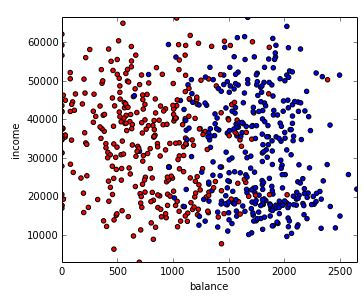
\includegraphics[width=0.6\linewidth]{sklclass3}
% %\end{center}
% %\end{frame}
% %
% %%%%%%%%%%%%%%%%%%%%%%%%%%%%%%%%%%%%%%%%%%%%%%%%%%%%%%%%%%%%%%%%%%%%%%%%%
% %\begin{frame}[fragile]\frametitle{}
% %\begin{center}
% %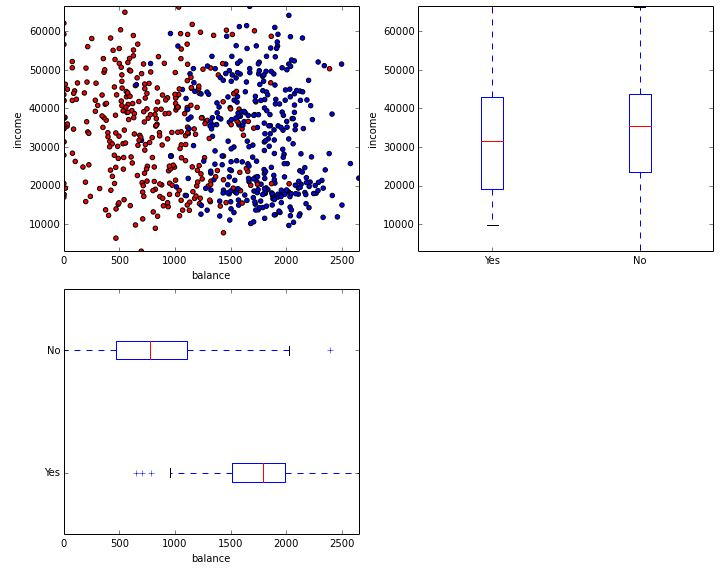
\includegraphics[width=0.8\linewidth]{sklclass4}
% %\end{center}
% %\end{frame}
% %
% %%%%%%%%%%%%%%%%%%%%%%%%%%%%%%%%%%%%%%%%%%%%%%%%%%%%%%%%%%%%%%%%%%%%%%%%%
% %\begin{frame}[fragile]\frametitle{Simple Approach - Linear Regression}
% %\begin{itemize}
% %\item A simple approach to binary classification is to simply encode default as a numeric variable with 'Yes' == 1 and 'No' == -1; fit an Ordinary Least Squares regression model and use this model to predict the response as 'Yes' if the regressed value is higher than 0.0 and 'No' otherwise. 
% %\item The points for which the regression model predicts 0.0 lie on the so-called decision surface - since we are using a linear regression model, the decision surface is linear as well.
% %\end{itemize}
% %\end{frame}
% %
% %
% %%%%%%%%%%%%%%%%%%%%%%%%%%%%%%%%%%%%%%%%%%%%%%%%%%%%%%%%%%%%%%%%%%%%%%%%%
% %\begin{frame}[fragile]\frametitle{}
% %\begin{center}
% %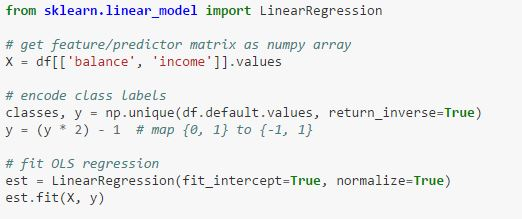
\includegraphics[width=0.6\linewidth]{sklclass6}
% %\end{center}
% %\begin{center}
% %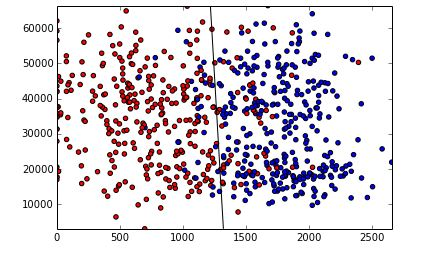
\includegraphics[width=0.4\linewidth]{sklclass7}
% %\end{center}
% %\begin{itemize}
% %\item Points that lie on the left side of the decision boundary will be classified as negative; 
% %\item Points that lie on the right side, positive. 
% %\end{itemize}
% %%The implementation of plot_surface can be found in the Appendix. 
% %\end{frame}
% %
% %%%%%%%%%%%%%%%%%%%%%%%%%%%%%%%%%%%%%%%%%%%%%%%%%%%%%%%%%%%%%%%%%%%%%%%%%
% %\begin{frame}[fragile]\frametitle{Confusion Matrix}
% %\begin{itemize}
% %\item We can assess the performance of the model by looking at the confusion matrix - a cross tabulation of the actual and the predicted class labels. 
% %\item The correct classifications are shown in the diagonal of the confusion matrix. The off-diagonal terms show you the \textbf{classification errors}. 
% %\item A condensed summary of the model performance is given by the \textbf{misclassification rate} determined simply by dividing the number of errors by the total number of cases.
% %\end{itemize}
% %\end{frame}
% %
% %%%%%%%%%%%%%%%%%%%%%%%%%%%%%%%%%%%%%%%%%%%%%%%%%%%%%%%%%%%%%%%%%%%%%%%%%
% %\begin{frame}[fragile]\frametitle{Confusion Matrix}
% %\begin{center}
% %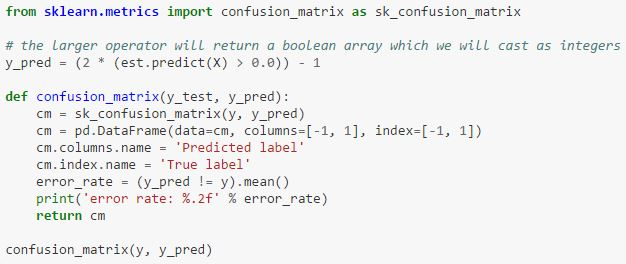
\includegraphics[width=0.8\linewidth]{sklclass8}
% %\end{center}
% %\begin{center}
% %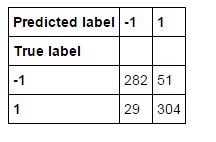
\includegraphics[width=0.6\linewidth]{sklclass9}
% %\end{center}
% %\end{frame}
% %
% %%%%%%%%%%%%%%%%%%%%%%%%%%%%%%%%%%%%%%%%%%%%%%%%%%%%%%%%%%%%%%%%%%%%%%%%%
% %\begin{frame}[fragile]\frametitle{Cross Validation}
% %\begin{itemize}
% %\item In this example we are assessing the model performance on the same data that we used to fit the model. 
% %\item This might be a biased estimate of the models performance, for a classifier that simply memorizes the training data has zero training error but would be totally useless to make predictions.
% %\item  It is much better to assess the model performance on a separate dataset called the test data.
% %\item  Scikit-learn provides a number of ways to compute such held-out estimates of the model performance.
% %\item One way is to simply split the data into a \textbf{training set} and \textbf{testing set}.
% %\end{itemize}
% %\end{frame}
% %
% %%%%%%%%%%%%%%%%%%%%%%%%%%%%%%%%%%%%%%%%%%%%%%%%%%%%%%%%%%%%%%%%%%%%%%%%%
% %\begin{frame}[fragile]
% %\begin{center}
% %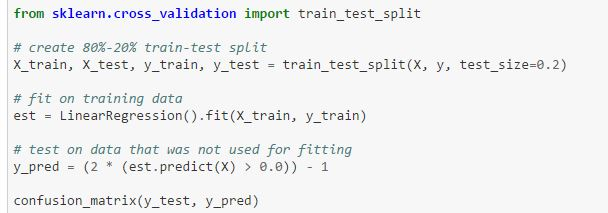
\includegraphics[width=0.8\linewidth]{sklclass10}
% %\end{center}
% %\begin{center}
% %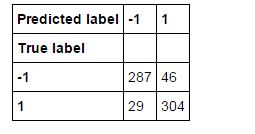
\includegraphics[width=0.6\linewidth]{sklclass11}
% %\end{center}
% %\end{frame}
